%-------------------------------------------------------------------------------
\section{Data Disguising}
%-------------------------------------------------------------------------------
\begin{figure}[t!]
    \centering
    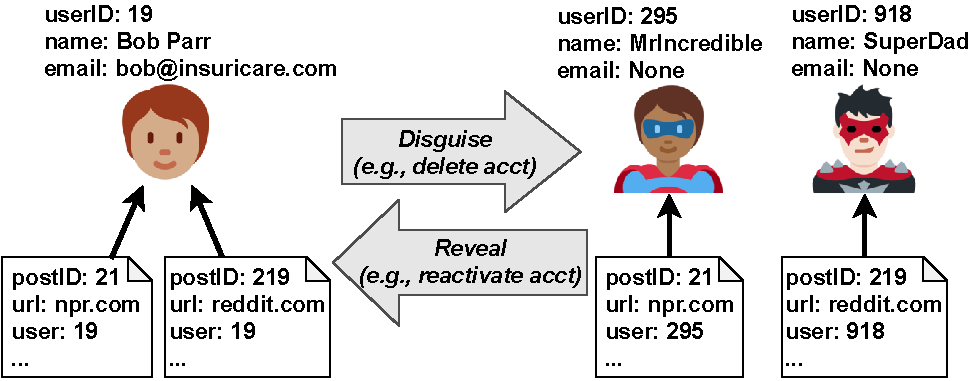
\includegraphics[width=0.5\textwidth]{img/disguises}

    \caption{Disguises move the target object (in this example, a user Bob) from an identity-revealing
    guise to privacy-preserving guises.}
    \label{fig:example}
\end{figure}

%\lyt{TODO (Frans): drive w/explicit example of table rows and foreign key relationships, too
%abstract. Start with Figure~\ref{fig:arch}?}

\begin{figure*}[t!]
    \centering
    \footnotesize
\begin{tabular}{@{}c|c|c|c@{}}
\textbf{User Transformation Spec} & \textbf{User Object} & \textbf{Guise 1} &
    \textbf{Guise 2} \\
\begin{lstlisting}[language=Rust]
"id":       IDAttribute,
"name":     Gen(Random),
"active":   Gen(Default(false)),
"darkmode": CopyAll,
"notifs":   CopyOnce+Gen(Default(false)),
"tag_id":   GenForeignKey,
\end{lstlisting}
    &
\begin{lstlisting}[language=Rust]
"id":       19,
"name":     BobParr,
"active":   true,
"darkmode": false,
"notifs":   true,
"tag_id":   11
\end{lstlisting}
&
\begin{lstlisting}[language=Rust]
"id":       295,
"name":     MrIncredible,
"active":   false,
"darkmode": false,
"notifs":   true,
"tag_id":   81483
\end{lstlisting}
&
\begin{lstlisting}[language=Rust]
"id":       918,
"name":     SuperDad,
"active":   false,
"darkmode": false,
"notifs":   false,
"tag_id":   15592
\end{lstlisting}
\end{tabular}
    \caption{Creating two guises of an example user (of a synthetic application schema).}
    \label{fig:guises}
\end{figure*}


%
The key idea behind \emph{data disguising} is to associate multiple \emph{guises} with a target
data object. Guises vary in how they reveal identities or preserve privacy.
%
Objects move between different guises by means of privacy transformations.
%
Figure~\ref{fig:example} illustrates this with the example of user account deletion.
%
When his account is active, user Bob's profile is associated with his true identity and all his
contributions to the site (an identity-revealing guise).
%
When Bob deletes his account, his profile and contributions move to different, privacy-preserving
guises: his name has been anonymized, his email address has been redacted, and his contributions
have been decorrelated and attributed to individual, unidentified user guises.
%

%
Data disguising builds on the existing structure of web applications.
%
Web applications are often structured as object graphs, either explicitly~\cite{tao, delf},
through an object-relational model (ORM)~\cite{orm}, or implicitly via foreign keys (edges)
between tables (vertices) in relational databases.
%
Data disguises transform this object graph.
%

%
The application developer writes a disguise specification for each privacy transformation needed
in the application.
%
This specification is a declarative statement similar to a relational schema, with entries for
graph vertices (objects) and directed edges (relationships between pairs of objects)
to be transformed (see \S\ref{sec:policies}).
%
We assume that:
\begin{enumerate}[nosep]
  \item developers use their domain knowledge to write correct and complete disguises;
    %\lyt{a bit worried about ``complete'' here}
  \item application code handles the different guises appropriately (\eg in
    displaying them); and
  \item different guises of the same object have the same structure (\eg they can be
    rows in the same table).
\end{enumerate}
%
A data disguising tool takes the disguise specification and turns it into storage operations that
apply the transformation (disguise) or its reverse (reveal).
%
% Malte: I don't think the following is fundamental
%The tool proxies application queries to its data storage, and exposes ``DISGUISE'' and
%``REVERSE DISGUISE" operations that invoke the disguise on transformation-triggering events
%(\eg user account deletion, data timeout, etc.).
%\lyt{This repeats the intro currently; perhaps we want to put it only there?}
%

%\begin{enumerate}[nosep]
  %\item application developers use their domain knowledge to write correct and complete
    %disguise specifications;
%\item \lyt{Not sure we need this?} application code invokes disguises via the disguising tool's API on
 %   transformation-triggering events (\eg user account deletion, data timeout, etc.); and
%  \item application code is prepared to handle the different guises appropriately (\eg in displaying
%      them); guises have the same structure as application objects (\eg exist as rows in existing
%        application tables).
%\end{enumerate}
%
At any given moment, an application's data object graph comprises a mix of
identity-revealing guises and privacy-preserving ones. Privacy transformations split
and combine individual guises when triggered.
%
%Using their application expertise, the developer selects from a menu of possible transformations
%(Section~\ref{sec:policies}) that can be performed on objects and object graph edges.
%The data disguise consists of the chosen set of transformations, and determines the
%structure of the object graph after a target (\eg the unsubscribing user) is disguised.
%
%Disguising a target object creates \emph{guises}---transformed versions and/or copies of the target.
%Disguising requires object deletion and anonymization: guises help maintain referential integrity
%when data is deleted, and transform objects into anonymized forms.  Guises additionally decorrelate
%other objects from the target: for example, a new guise for the user can be created in the users
%table, and the foreign key relationship from a row in the posts table rewritten to point this guise,
%to decorrelate the post from the user.

%-------------------------------------------------------------------------------
\section{Specifying Data Disguises}
%-------------------------------------------------------------------------------
\label{sec:policies}

%
Data disguises involve transformations on object types and edge types in the
application object graph.
%
A disguising tool applies these transformations by traversing the graph starting from a
developer-specified target object, such as a deleted user.
%
%The developer chooses one transformation for each object type, and
%one for each edge type.
%Object type transformations specify how to transform a template object of that type into guises; edge type
%transformations specify whether to delete, retain, or decorrelate edges of that type.
%where decorrelation replaces the edge with edges to guises.

%We next describe a menu of object and edge transformations sufficient to write disguises for the
%privacy transformations in Section~\ref{sec:survey}.

\subsection{Creating Guises for Objects}
\label{sec:guises}
%
To create a guise from an object, developers specify how to transform attributes of the
object into guise attributes.
%
Figure~\ref{fig:guises} shows an example, producing guises for user objects.
%
User objects have identifier \texttt{id}; a reference \texttt{tag\_id}
forms an edge in the graph (a foreign key constraint to tag objects).
%

%An object has three kinds of attributes: a unique identifier attribute; value
%(non-referential) attributes such as timestamps or usernames; and edge (\eg foreign key)
%attributes that refer to other objects.
%


%
Guises always have unique, random identifiers.
%
Developers choose how to create other guise attributes, selecting from among the following:
%
\paragraph{(1) Copy object content.}
%
Guises of the same object all share the object's attribute values.
%
If the attribute is an edge attribute (\eg a foreign key column), all guises will have
edges to the same object.
%
%
Copying allows developers to retain the object's content, without worrying about how to
synthesize attribute values for guises.
%
%However, this should only be chosen if guise attribute
%values cannot be generated, or if this attribute says little about the true identity of the
%entity.
For example, in Figure~\ref{fig:guises} the \texttt{darkmode} attribute is copied in
all guises.
%; the \texttt{darkmode} attribute reveals very little about the underlying user's
%identity.

\paragraph{(2) Generate new content.}
%
To create new attributes, developers specify whether the guise's value should be random,
a default value, or generated from the object's attribute value via a custom function (\eg hashing 
the value).
%
Figure~\ref{fig:guises} illustrates an example of random (\texttt{name}) and default
(\texttt{active}) generated value attributes.
%
%
Creating new guise edge attributes (\eg new foreign key relationships) requires
creating a new guise for the referenced object in order to maintain referential
integrity;
the data disguise rewrites the edge to point to the new guise.
%
In Figure~\ref{fig:guises}, creating two user guises requires creating two
tag guises, and the tag guises' identifiers become the user guises' foreign keys.
%

\paragraph{(3) Copy object content, but only once.}
%
One guise copies the attribute value from the object, but all other guises generate new
values (as described above).
%
\texttt{notifs} in Figure~\ref{fig:guises} illustrates how the attribute is copied once.
%
This enables the application to retain the original object semantics (\eg a count of how many
users want notifications) without creating duplicates.
%

\subsection{Transforming Edges Between Objects}
\label{design:edgepol}
%
Edge transformations specify how a disguise restructures the object graph as it
recursively traverses edges from the target.
%
% SOURCE = CHILD
% DEST = PARENT
Edges have a \emph{source} object and a \emph{destination} object, where the source references
the destination (\eg via a foreign key column in a relational database).
%
The developer specifies transformations for each edge type, choosing from the following:
%
\begin{enumerate}[nosep]
    %
    \item \textbf{Retain} edges of this type.
    %
    Transforms both source and destination objects into a single guise each.
    %
    \item \textbf{Decorrelate} edges of this type.
    %
    Creates one guise of the destination object for each of the sources; replaces each source's
    edge to the destination with an edge to that unique guise.
    %
    \item \textbf{Delete} edges of this type.
    %
    Transforms the destination object into a single guise; removes the source and its descendants
    if otherwise unconnected.
    %
\end{enumerate}
%
An optional argument enables conditionally-applied edge transformations, \eg removing only
user-created tags, or removing tags only until the user's papers comprise less than
$10$\% of tagged papers. %; or transforming only in the child-parent direction.
%

\subsection{An Example Disguise}
\label{design:eg}
%
Consider disguising Bob when he deletes his HotCRP account.
%
Bob would prefer his papers and reviews to be unlinked from his identity.
%
HotCRP, on the other hand, would like to retain paper and review information that other users
find useful.
%
A careful selection of edge and object transformations achieves both.
%

%
To decorrelate reviews from Bob, the disguise \texttt{Decorrelate}s user-to-review edges.
%
This requires transforming Bob into one unique user guise per review.
%
The disguise generates guise attribute values using suitable defaults;
%
in particular, HotCRP users' \texttt{disabled} attribute is set for the guises,
ensuring that guises have no permissions and never review papers.
%

%
Bob is further linked to papers through conflicts, which can indicate coauthorship or a
reviewer conflict.
%
These conflicts are not reassigned to the new guises, since preserved
conflicts could reidentify Bob as the likely author of a review. Thus, the
conflict edges that link a disguised user to papers need a \texttt{Delete} annotation.
%
%% Edge directionality matters here: paper-to-conflict edges should not be removed, as doing so
%% could incorrectly allow conflicted users to see the paper!

The disguise \texttt{Retain}s all other edge types, ensuring that review and paper
artifacts remain correctly linked. Active reviewers still see the correct paper for their reviews,
and active authors see the correct reviews for their papers, albeit potentially authored by
anonymous, unlinkable guises of the original reviewer.
%
%Review and paper guises copy the original object, retaining paper and review information.
%
%\ms{Does this mean duplicate papers/reviews can show up?}

%
Unlike the current real-world HotCRP account deletion policy~\cite{hotcrp:privacy}, which
deletes all objects belonging to Bob, this disguise strikes a balance between decorrelating
Bob's identity from his reviews and papers, and maintaining useful information for other
HotCRP users.
%
Furthermore, it is easy to imagine extending this disguise to automatically disguise Bob
after some time (\eg 2 years after the conference), protecting his future research career
by hiding youthful reviewing sins.
%

%%%%%%%%%%%%%%%%%%%%%%%%%%%%%%%%%%%%%%%%%%%%%%%%%%%%%%%%%%%%%%%%%%%%%%%%%%%%%%%%%%%%%%%%%%%%%%%%%%%%%%
%%%%%%%%%%%%%%%%%%%%%%%%%%%%%%%%%%%%%%%%%%%%%%%%%%%%%%%%%%%%%%%%%%%%%%%%%%%%%%%%%%%%%%%%%%%%%%%%%%%%%%
%%%%%%%%%%%%%%%%%%%%%%%%%%%%%%%%%%%%%%%%%%%%%%%%%%%%%%%%%%%%%%%%%%%%%%%%%%%%%%%%%%%%%%%%%%%%%%%%%%%%%%

\iffalse
%By default, all \emph{sensitive} entities---entities transitively connected via
%parent-child edges to the mask's target entity---transform into with ghost entities.
%For example, in Figure~\ref{fig:edgepol}a, all reviews and papers of the unsubscribing user are by
%default replaced by ghosts.

%Any parent of a sensitive child is ghosted as well. This is not actually true; we retain the
%original parent entity, but allow it to be decorrelated
%\lyt{Child-to-Parent edges can have different ghost
%generation policies + edge policies than Parent-to-Child edges. I'm not sure if we should mention
%that here (seems too detailed?)}

\paragraph{Child-Parent Edge Transformations.}
Data masks also allow the developer to specify edge transformations in the child-parent direction,
namely from sensitive children to parents that are not descendants of the user.
%
For example, papers have both tags and users as parents. If an unsubscribed user authors all papers
with a particular tag, the developer may realize that the tag can reidentify the user, and want to
decorrelate the paper from the tag.

Because parents of sensitive children may have non-sensitive children (\eg many papers may share
tags with the user's papers), decorrelation and delete transformations in the child-parent direction
take a \textbf{sensitivity threshold} as an argument, which tells the mask how many edges need to be
decorrelated or deleted.

In the paper-tag example, a reasonable sensitivity threshold
might be $0.1$: fewer than 10\% of all papers with a specific tag key should be correlated with an
(unsubscribed) user.  Figure~\ref{fig:sensitivity} shows an example in which paper-tag edges are
decorrelated to meet a threshold of 0.5.

\paragraph{Edge Transformation Filters}
For decorrelation or delete transformations (in either parent-child or child-parent directions), the
developer can additionally specify an \textbf{edge filter}. The filter takes the parent and child
entities of the edge as inputs, and returns whether the entities satisfy the filter. If yes, the
edge is decorrelated or deleted; otherwise, the edge is retained.
%
For example, perhaps we want to remove tags from a user's papers (decorrelate paper-tag edges)
\emph{only if} the tags were created by the unsubscribing user.
\fi

%%%%%%%%%%%%%%%%%%%%%%%%%%%%%%%%%%%%%%%%%%%%%%%%%%%%%%%%%%%%%%%%%%%%%%%%%%%%%%%%%%%%%%%%%%%%%%%%%%%%%%
%%%%%%%%%%%%%%%%%%%%%%%%%%%%%%%%%%%%%%%%%%%%%%%%%%%%%%%%%%%%%%%%%%%%%%%%%%%%%%%%%%%%%%%%%%%%%%%%%%%%%%
%%%%%%%%%%%%%%%%%%%%%%%%%%%%%%%%%%%%%%%%%%%%%%%%%%%%%%%%%%%%%%%%%%%%%%%%%%%%%%%%%%%%%%%%%%%%%%%%%%%%%%

\iffalse
\sys also handles user data management and storage.
While unsubscribing a user, \sys tracks all deletions and modifications to the database.
\sys encrypts this log with a per-user key, and stores this encrypted
blob in a dedicated application datastore (Figure~\ref{fig:arch}, step 5). The user key is secret-shared using a (2, 3)
threshold scheme~\cite{secretsharing} between the user, \sys, and a trusted third party (\eg
Amazon S3), so that the user can authorize \sys and the third party to restore the key if
the user forgets their share.
%Alternatively, the key can also be password-encrypted, which relies
%on the user not forgetting their password.
The user can optionally choose to store this encrypted data themselves
%(or in a third party cloud provider),
and be in charge of providing their data and key to \sys to decrypt the data upon
resubscription.

To resubscribe, a user authorizes the decryption of their data and associated metadata by
providing their share of the key (or authorizing a trusted third party to reconstruct the secret
with the application). \sys decrypts the data with the key, and systematically reverses
the modifications made during unsubscription, restoring removed entities and correlations between
entities.
\fi

%%%%%%%%%%%%%%%%%%%%%%%%%%%%%%%%%%%%%%%%%%%%%%%%%%%%%%%%%%%%%%%%%%%%%%%%%%%%%%%%%%%%%%%%%%%%%%%%%%%%%%
%%%%%%%%%%%%%%%%%%%%%%%%%%%%%%%%%%%%%%%%%%%%%%%%%%%%%%%%%%%%%%%%%%%%%%%%%%%%%%%%%%%%%%%%%%%%%%%%%%%%%%
%%%%%%%%%%%%%%%%%%%%%%%%%%%%%%%%%%%%%%%%%%%%%%%%%%%%%%%%%%%%%%%%%%%%%%%%%%%%%%%%%%%%%%%%%%%%%%%%%%%%%%

\iffalse
\subsection{\sys's Execution Algorithm}
\begin{figure*}[ht!]
    \centering
    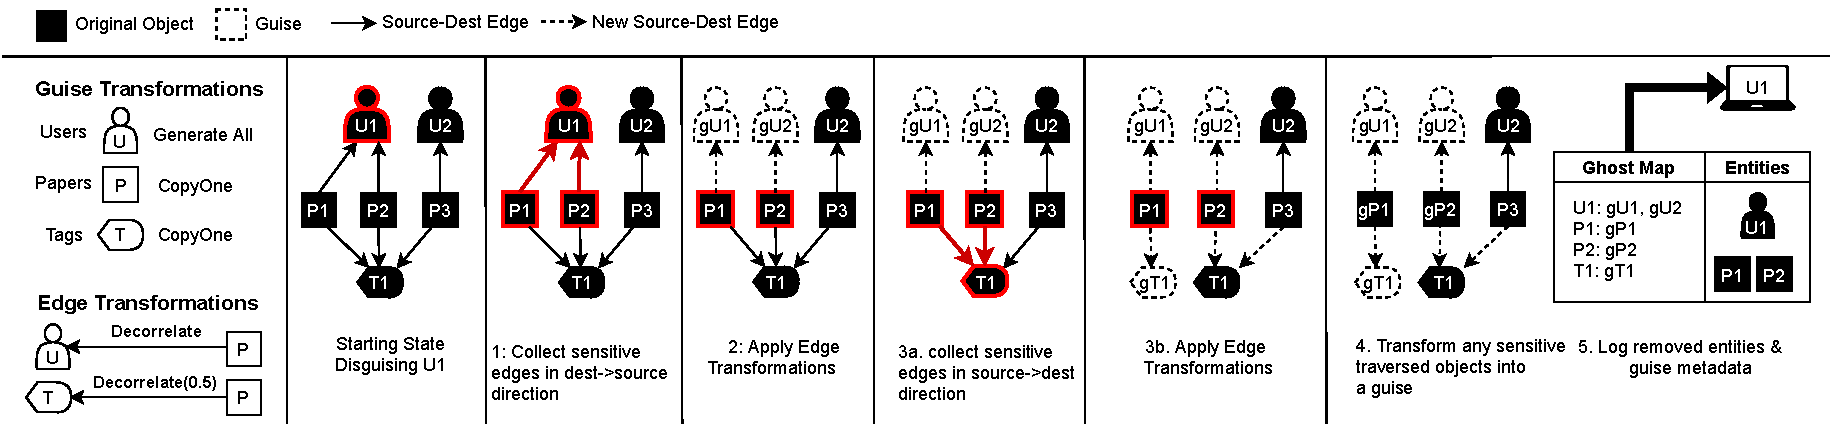
\includegraphics[width=\textwidth]{img/algo}

    \caption{Stages of \sys's execution when unsubscribing user U1. Entities and edges detected as
    sensitive are outlined in red. Only the part of the entity graph relevant to unsubscription is shown.
    For simplicity, the specified guises policies apply for all attributes
    of the entity: a black ghost entity indicates that it is a full clone of the original.
    New edges indicates that the edge (foreign-key) value of the child has been changed to
    point to the specified parent.\\
    In this example, \sys decorrelates paper-tag edges only enough that the proportion of sensitive papers
    is at most the sensitivity threshold of 0.5, retaining one correlation between a sensitive
    paper P2 and the parent tag T1, and decorrelating the other sensitive paper P1 from the tag.}
    \label{fig:algo}
\end{figure*}


Given an application's schema and unsubscription policy, and an entity to be decorrelated as input,
\sys executes unsubscription as follows. Figure~\ref{fig:algo} illustrates each step.
\begin{enumerate}
    \item \textbf{Parent-Child Traversal:} \sys traverses the entity graph starting from the input entity,
        going down parent to child edges (and halting if it detects a cycle).
        \sys collects traversed edges as it traverses the graph.

    \item \textbf{Parent-Child Edge Policy Application:}
        Post-traversal, \sys acts on each collected edge instance according to the specified
        decorrelation relationship policy for that edge's type.

        \sys takes all edges of every unique parent entity, and applies policies as appropriate.
        Note that any sensitivity threshold less than $1$ requires that \emph{all} edges be decorrelated or
        deleted, depending on the developer's specified choice: all the children of this parent are
        sensitive due to the nature of \sys's parent-child traversal.

        Any edges that should be deleted removes the child entity and any descendants.
        \sys generates new ghost parents using the real parent as template for any edges that should
        be decorrelated, and rewrites the child's edge attribute to be the ghost parent's
        identifier. If any edges are retained, \sys generates a ghost parent entity to replace the
        parent.

    \item \textbf{Child-Parent Edge Policy Application:}
        Next, \sys takes the children of all traversed edge instances, and considers the set of
        edges from these children to other parents \emph{not} traversed by \sys during the first
        traversal phase. In other words, these children have multiple parents, at least one of which
        is transitively connected to the input entity.

        Intuitively, children of edges traversed by \sys share a connection with the initial
        entity being decorrelated. Edges \emph{from} these children to other parent entities may
        thus leak sensitive identifying information.

        \sys acts on these child-parent edges according to the specified edge policy for each edge's
        type. For each unique parent, \sys limits the proportion of edges of each type that connect
        to sensitive entities (the children of traversed edge instances) to below the policy's
        sensitivity threshold by either decorrelating or deleting the children.
        If \sys retains any edges from sensitive children to the real parent, then \sys generates a
        ghost parent entity to replace the parent.

        Note that unlike the previous steps, this step considers edges from parents that may have
        many non-sensitive children (\eg a particular tag may correlate with many stories by various
        authors).  \sys therefore may retain edges to sensitive children when given a sensitivity
        threshold less than 1 and greater than 0, unlike in the previous step.

        \sys optionally allows developers to specify that edges have weaker or stronger edge
        policies in the child-to-parent direction than in the  parent-to-child direction. Weaker
        policies---higher sensitivity thresholds---allow \sys to retain links if \emph{only the
        child} is sensitive, but decorrelate or remove the link if \emph{both} the child and parent
        are sensitive. For example, perhaps a user wants to ensure that they are decorrelated from
        their reviews, but correlations between the review and the the paper authors can still be
        retained.

        Stronger policies may specify that the parent connected to sensitive children should
        decorrelate \emph{all} correlations to the paper even from non-sensitive correlations.
        Developers specify such a policy with a sensitive threshold of -1. For
        example, perhaps the set of users with review conflicts to the paper can identify the
        author, even if the author is decorrelated from the paper. We see an example of this in
        Section~\ref{sec:hotcrp_example} (Figure~\ref{fig:pcs}).

    \item \textbf{Anonymizing Leaf Children:}
        If any sensitive children that are leaves (have no children) remain, \sys generates a ghost child entity to replace this leaf.

        In Figure~\ref{fig:algo}, step 4, P1 and P2 are both leaves. \sys generates ghosts for both
        these papers: since these papers have \texttt{CloneOne} guises policies, ghost papers gP1
        and gP2 are identical to P1 and P2, and retain the edge attributes linking them to their
        respective parent tags and users.

    \item \textbf{Returning User Data:} \sys collects all removed entities that have either been
        replaced by ghost entities, or deleted entirely from the graph. \sys also records all
        generated ghost entity identifiers, and which ghost entities replaced which real entity.
        \sys returns both the removed entity data and this ghost entity metadata to the user.
\end{enumerate}

Note that \sys must decide \emph{which} ghost clones the template entity's attributes when the
developer selects a \texttt{CloneOne} guises policy for one or more attributes. \sys always
associates the cloned ghost with as many non-sensitive entities as possible. For example, as shown
in Figure~\ref{fig:algo} step 3b, if \sys decorrelates sensitive papers from a parent tag with a
\texttt{CloneOne} policy, \sys chooses the ghost tag that remains associated with non-sensitive
papers to be the clone. This decision ensures that any unsensitive application
data remain as unaffected as possible when disguising another entity.
To optimize
\texttt{CloneOne} policies, \sys can simply retain the original template entity instead of producing
a cloned ghost.
%\sys provides a menu of unsubscription policy choices that allow developers to choose how to
%\emph{ghost} individual data record content, and how to \emph{decorrelate} sensitive correlations.
%Specifying the policy requires nothing more than the application schema: guises policies act on
%application datatables and on foreign key relationships between tables.
%Table column values can be ghosted---removed, anonymized, or modified---in application-specific
%ways; and correlations can be broken, removed, or desensitized by adding noise. This gives
%developers the flexibility to specify fine-grained policies that properly de-identify a user, while
%retaining data as necessary for the application.

%\sys must pinpoint exactly which data and correlations may be
%identity-sensitive, and allow developers to specify exactly what the post-unsubscription state of
%this data should be.

\fi

